\section{Analyse von Funktion F230(Bib\TeX -Export)}
Diese Funktion gehört zur Komponente \textbf{View:Export}. Die für diesen Export nötigen Informationen sind vollständig in der Datenbank enthalten und müssen mit Django ermittelt werden. Die so erhaltenen Daten werden dem Benutzer in einer View im \BibTeX -Format zum Kopieren angezeigt. Verdeutlicht wird dies in dem Sequenzdiagramm \ref{fig:BibTeX-Export}.

\begin{figure}[h]
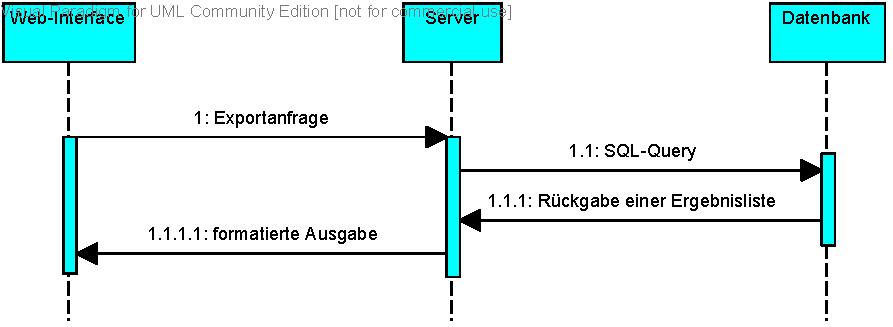
\includegraphics[width=0.8\linewidth]{bilder/Seq-BibTex.pdf}
\caption[BibTeX-Export]{BibTeX-Export}
\label{fig:BibTeX-Export}
\end{figure}

\section{Analyse von Funktion F231(Universitätsbibliothek-Export)}

Diese Funktion muss in einer extra Klasse dargestellt werden. Die für diesen Export nötigen Informationen sind vollständig in der Datenbanken enthalten und müssen mittels einer direkten Datenbankabfrage ermittelt werden. Diese Daten werden durch eine Funktion in das richtige Format gebracht und in einem vom Benutzer vorher gewählten Dateipfad in einem Allegro kompatiblen Format gespeichert. Dieses Sequenzdiagramm ist strukturell genauso wie das für den \BibTeX -Export, nur das auf eine andere Weise ausgegeben wird. Deswegen wird dies hier weggelassen. Diese Komponente gehört zur \textbf{View}.


\section{Analyse von Funktion F300(Benutzerverwaltung)}
Alle Informationen zu den Benutzern werden in einer Datenbank gespeichert. Änderungen an bestehenden Benutzern und das Hinzufügen neuer Benutzer wird durch ein Webformular von einem Benutzer mit ausreichenden Rechte eingeleitet. Mithilfe von Django werden die Informationen aus dem Formular gelesen und alle Änderungen in der Datenbank eingetragen. Das Sequenzdiagramm ist trivial, da nur einfach Frage/Antwort-Vorgänge zwischen Server und Datenbank stattfinden. Diese Komponente gehört zur Komponente \textbf{Admin}.

\section{Analyse von Funktion F301(Rechtezuweisung für Rollen)}
Die Rechte einer Rolle werden in einer eigenen Tabelle der Datenbank gespeichert. Ein Benutzer mit ausreichenden Rechten kann über ein Webformular Änderungen eingeben. Diese Änderungen werden mithilfe von Django aus dem Webformular ausgelesen und in der Tabelle der Datenbank gespeichert. Das Sequenzdiagramm ist trivial, da nur einfach Frage/Antwort-Vorgänge zwischen Server und Datenbank stattfinden. Diese Funktion gehört zur Komponente \textbf{Admin}.

\section{Analyse von Funktion F302(Benutzer Rolle(n) zuweisen)}
Die Rollen eines Benutzer werden in einer speziellen Tabelle in der Datenbank gespeichert. Ein Benutzer mit ausreichenden Rechten kann über ein Webformular Änderungen eingeben. Diese Änderungen werden mithilfe von Django aus dem Formular ausgelesen und in der entsprechenden Datenbank gespeichert. Das Sequenzdiagramm ist trivial, da nur einfach Frage/Antwort-Vorgänge zwischen Server und Datenbank stattfinden. Diese Funktion gehört zur Komponente \textbf{Admin}.
